\section{Zuständigkeiten (TiK)}
\label{section_zustaendigkeiten}
In diesem Kapitel wird auf die Zuständigkeiten in Bezug auf die Informationsbereitstellung an der Hochschule Emden/Leer näher eingegangen. Es wird dargestellt, welche Bereiche bereits zentral an der Informationsbereitstellung beteiligt sind. Ebenso wird auf die Besonderheiten einzelner Fachbereiche, zentraler Einrichtungen und dem Präsidium detaillierter eingegangen (siehe Abbildung \ref{fig_organigramm_HS}). 

\begin{figure}[h!]
	\centering
	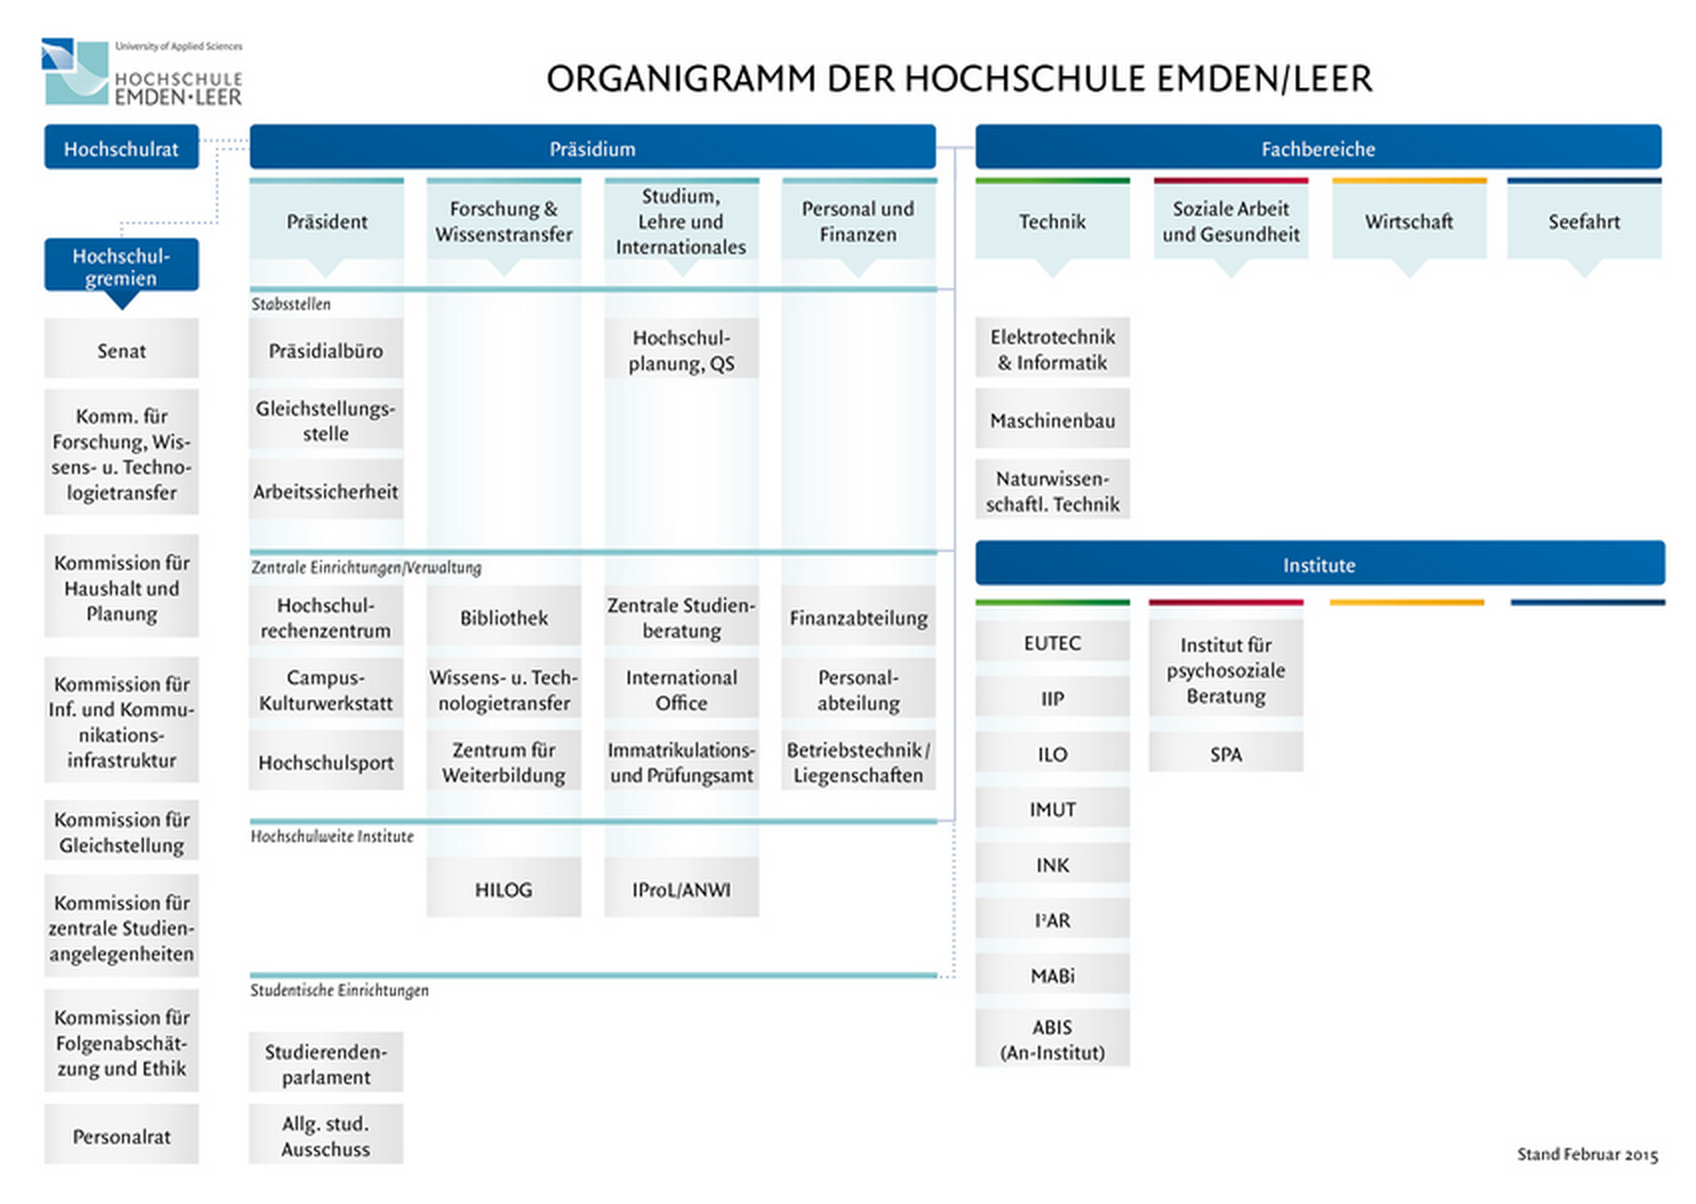
\includegraphics[width=14cm]{kapitel/gruppe2/bilder/organigramm_HS}
	\caption{Organigramm der Hochschule Emden/Leer}
	\label{fig_organigramm_HS}
\end{figure}

Nachfolgend wird ein Überblick über die IT-Systeme gegeben, welche sowohl von Mitarbeitern als auch Studierenden verwendet werden (siehe Abbildung  \ref{fig_zentrale_systeme}). Bei einigen zentralen Systemen ist bereits eine Authentifizierung über Single Sign On (SSO) gegeben (siehe Kapitel \ref{realisierung_der_serviceorientierung} auf Seite \pageref{realisierung_der_serviceorientierung}).

\begin{figure}[h!]
	\centering
	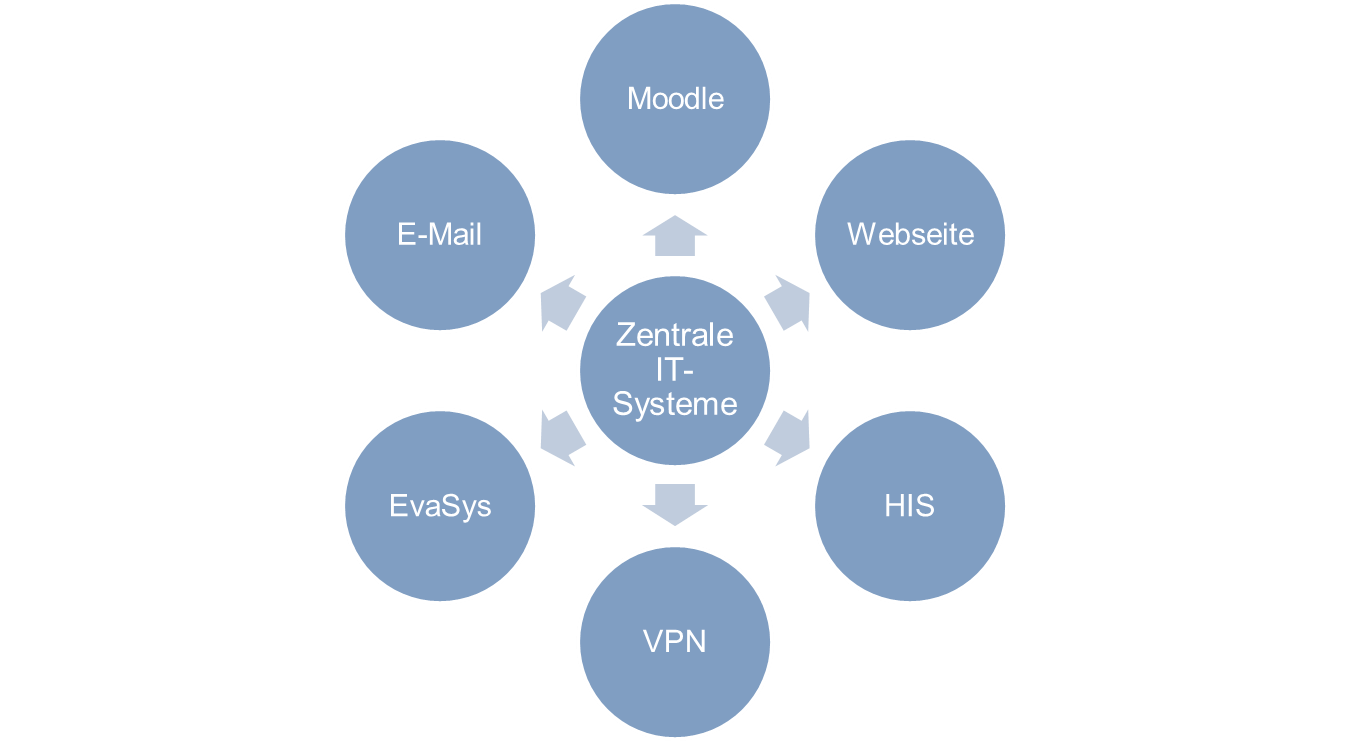
\includegraphics[width=14cm]{kapitel/gruppe2/bilder/zentrale_systeme}
	\caption{Zentrale Systeme für Mitarbeiter und Studenten}
	\label{fig_zentrale_systeme}
\end{figure}


\subsection{Fachbereiche}
Die einzelnen Fachbereiche sind unter anderem durch die Mitgliedschaft in Arbeitsgruppen in den Informationsbeschaffungsprozess involviert.

Alle Fachbereiche verfügen über die Berechtigung, relevante Informationen im System InfoSys darzustellen. InfoSys ist eine zentrale Plattform zur Darstellung von organisatorischen Informationen. Diese können direkt online auf der öffentlichen Webseite der Hochschule oder in den Eingangsbereichen der jeweiligen Fachbereiche vor Ort über entsprechende Monitore eingesehen werden. Es werden, nach Fachbereich sortiert, die wichtigsten Neuigkeiten als Newsticker dargestellt und der Zugriff auf alle Vorlesungspläne der Fachbereiche wird zur Verfügung gestellt, um so zügig auf organisatorische Inhalte zugreifen zu können (siehe Abbildung \ref{fig_InfoSys}). Aufbauend auf InfoSys wird eine selbst entwickelte Android-App zur Verfügung gestellt.

\begin{figure}[h!]
	\centering
	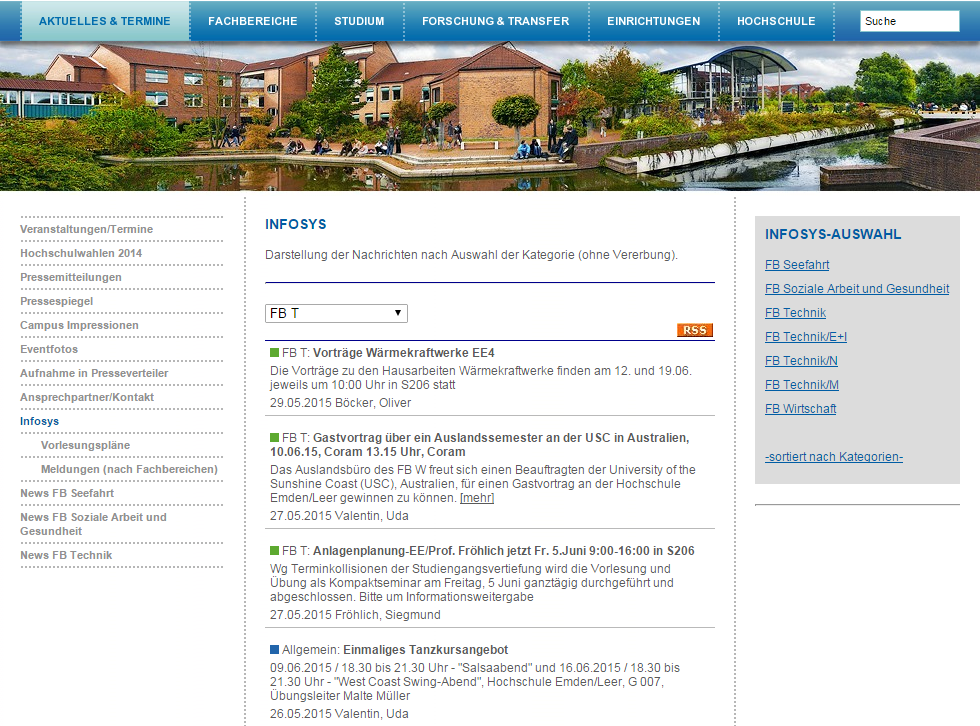
\includegraphics[width=14cm]{kapitel/gruppe2/bilder/InfoSys}
	\caption{Exemplarischer Screenshot vom InfoSys des Fachbereiches Technik}
	\label{fig_InfoSys}
\end{figure}

In den nachfolgenden Kapiteln wird auf die Besonderheiten der einzelnen Fachbereiche eingegangen.

\subsubsection{Seefahrt}
Der Fachbereich Seefahrt ist ein relativ kleiner Fachbereich, der nur am Standort Leer vertreten ist. Dieser Fachbereich verwendet kein zentrales System zur Vorlesung und Raumplanung, sondern eine eigenentwickelte Lösung. 

\subsubsection{Technik}
Eine Besonderheit dieses Fachbereiches ist es, dass für den Laborbetrieb ein paralleles Netz neben dem zentralen Netz der Hochschule betrieben wird. Da unter anderem der Bereich „IT-Sicherheit“ einen wichtigen Aspekt im Studiengang Informatik bildet, kommt es zu besonderen Konstellationen im Bereich der Forschung. Technik verwaltet ihr Netz selbst und ist somit autark vom allgemeinen Hochschulrechennetz. Es besteht jedoch eine enge Zusammenarbeit zwischen Technik (im speziellen E+I) und dem Rechenzentrum, so dass unter anderem gegenseitige Zugriffsrechte bestehen. 

\subsection{Präsidium}
\label{praesidium_label}

Das Präsidium, insbesondere mit dem Bereich zentrale Verwaltung, ist über  Arbeitsgruppen in den Informationsbeschaffungsprozess involviert. Zudem verfügt das Präsidium mit einer Stabsstelle über einen zentralen Bereich im Bezug auf die Repräsentation von Informationen.  Das Präsidialbüro ist unter anderem das Hochschulmarketing zuständig. Dem Präsidialbüro, welches als Stabstelle fungiert, ist ebenfalls der Bereich Presse- und Öffentlichkeitsarbeit zugeordnet. 

\subsection{Zentrale Verwaltung}
Die zentrale Verwaltung verwendet im Bereich Personalverwaltung und Finanzen ausschließlich SAP als Buchhaltungssystem. Zur Organisation der Lehr- und Vorlesungsplanung wird UNTIS Plus verwendet. Ebenso wird für die Urlaubsplanung, Zeiterfassung und das Gebäudeschließsystem ein eigenständiges System verwendet. Speziell für die Aufbereitung von Kennzahlen und Zahlen kommt eine Eigenentwicklung als BIS (Business Intelligence System) zum Einsatz. 

\subsubsection{Rechenzentrum}
Das Hochschulrechenzentrum der Hochschule ist stark in die Administration und Pflege der bestehenden Systeme zur Informationsbereitstellung involviert. Neben der Administration von bestehenden Systemen obliegt dem Hochschulrechenzentrum ebenfalls der Endkundensupport.

\subsection{Arbeitsgruppen zum Informationsaustausch und zur Informationsbereitstellung}
\label{subsection_arbeitsgruppen_informationsaustausch}
Die Zuständigkeiten an der Hochschule, bezüglich der Informationssammlung, Beschaffung und Aufbereitung von Informationen, ist bereits durch Arbeitsgruppen in wichtigen Bereichen geregelt. Durch das Interview mit dem Leiter des Hochschulrechenzentrums konnte ein Einblick in die bestehenden Gremien geschaffen werden. Diese treffen sich regelmäßig zum Informations-, Wissens- und Erfahrungsaustausch.

Es existieren drei Arbeitsgruppen, welche für die Informationsverteilung in den jeweiligen Bereichen relevant sind:

\begin{itemize}
	\item Zahlen, Daten und Fakten (ZDF)
	\item WEB
	\item Moodle
\end{itemize}

\subsubsection{Zahlen, Daten und Fakten (ZDF)}
ZDF setzt sich zusammen aus den Verwaltungsabteilungen Finanzen, Personal, Presse und Rechenzentrum. Dieses Gremium ist zuständig für die Erstellung und Aufbereitung von Kennzahlen. Dies können zum Beispiel aktuelle Kennzahlen zu eingeschriebenen Studierenden pro Studiengang sein.  ZDF ist für einen Unterbereich der offiziellen Webseite der Hochschule zuständig. Die Kennzahlen und Zahlen werden gruppenbasiert erstellt. Je nach Berechtigung werden Kennzahlen in unterschiedlichen Detailgraden dargestellt. So erhalten Dekane mehr Informationen als andere Mitarbeiter. Öffentlich zugänglich sind nur generische Kennzahlen. 

\subsubsection{WEB}
Es existiert eine Arbeitsgruppe, welche für die Gestaltung und den Inhalt der öffentlichen Webseite der Hochschule verantwortlich ist. In dieser Arbeitsgruppe sind aus jedem Fachbereich Repräsentanten mit einbezogen. Die Leitung des Web-Teams obliegt dem Präsidialbüro.\footnote{\url{http://www.hs-emden-leer.de/fileadmin/user_upload/Einrichtungen/Praesidialbuero/Organigramm_Praesidialbuero_Juli2013_01.pdf}}

\subsubsection{Moodle}
In der Arbeitsgruppe „Moodle“ sind sowohl Repräsentanten aus jedem Fachbereich als auch der Verwaltungsebene involviert. Da das Moodle E-Learning System mittlerweile als ein zentrales Moodle für alle Bereiche eingeführt wurde, haben die Mitglieder aus den Fachbereichen unter anderem das Recht, Kurse im Moodle freischalten zu können. Auf die E-Learning Plattform „Moodle“ wird detaillierter im Kapitel \ref{paragraph_moodle} auf Seite \pageref{paragraph_moodle} eingegangen.
